% ---------------------------------------------------------------
% Generated by Flowchart -> TikZ Studio
% Every coordinate below is derived from the editor diagram model.
% Safe to edit by hand, but regenerating will overwrite changes.
% ---------------------------------------------------------------

\documentclass[border=8pt]{standalone}
\usepackage[T1]{fontenc}
\usepackage[utf8]{inputenc}
\usepackage{xcolor}
\usepackage{tikz}
\usetikzlibrary{arrows.meta}

% ---- Colour definitions ----
\definecolor{fc12161C}{HTML}{12161C}
\definecolor{fc1F2933}{HTML}{1F2933}
\definecolor{fc7C8A9B}{HTML}{7C8A9B}

% ---- Style definitions ----
\tikzset{
  fcnode/.style={
    draw, inner sep=0pt, outer sep=0pt, align=center,
    line join=round, line cap=butt
  },
  fcpath/.style={line join=round, line cap=butt},
  fcedge/.style={line join=round, line cap=butt},
  fclabel/.style={inner sep=1.4pt, outer sep=0pt, align=center},
}

\begin{document}
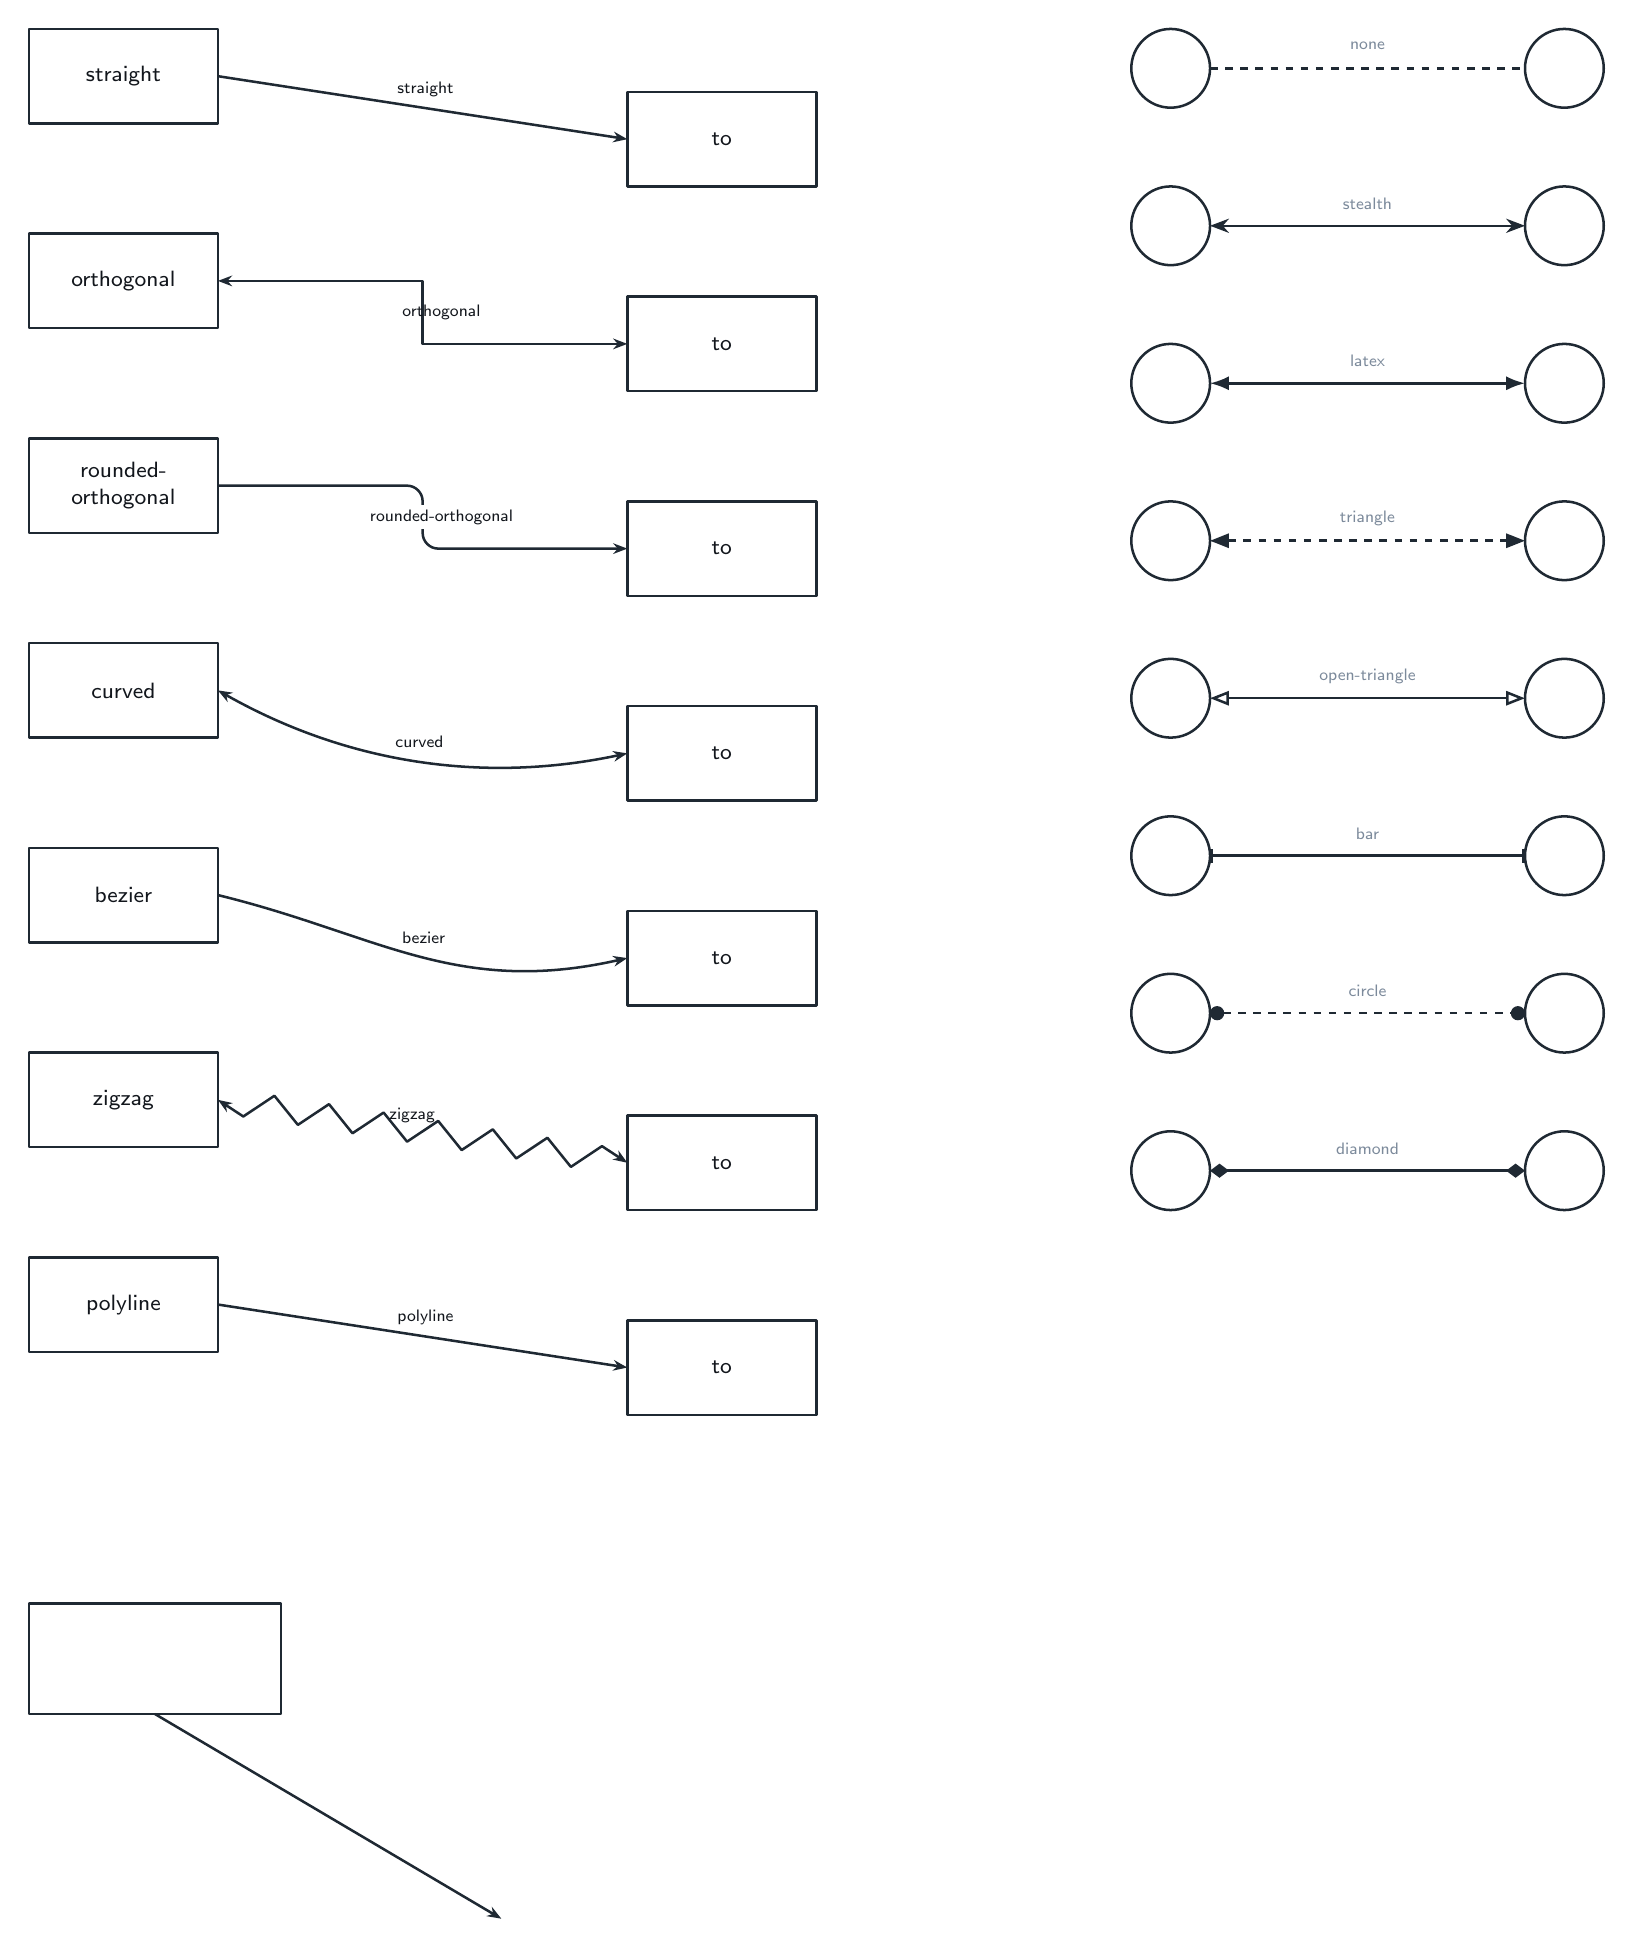
\begin{tikzpicture}[x=1cm, y=1cm]
  % ---- Nodes ----
  % a0 - Process "straight"
  \node[fcnode, shape=rectangle, minimum width=2.4cm, minimum height=1.2cm, draw=fc1F2933,
        line width=0.91pt, fill=white, font=\fontsize{7.97pt}{9.96pt}\selectfont\sffamily,
        text=fc12161C, align=center, text width=2.08cm] (a0) at (3.2,-2.6) {straight};
  % b0 - Process "to"
  \node[fcnode, shape=rectangle, minimum width=2.4cm, minimum height=1.2cm, draw=fc1F2933,
        line width=0.91pt, fill=white, font=\fontsize{7.97pt}{9.96pt}\selectfont\sffamily,
        text=fc12161C, align=center, text width=2.08cm] (b0) at (10.8,-3.4) {to};
  % a1 - Process "orthogonal"
  \node[fcnode, shape=rectangle, minimum width=2.4cm, minimum height=1.2cm, draw=fc1F2933,
        line width=0.91pt, fill=white, font=\fontsize{7.97pt}{9.96pt}\selectfont\sffamily,
        text=fc12161C, align=center, text width=2.08cm] (a1) at (3.2,-5.2) {orthogonal};
  % b1 - Process "to"
  \node[fcnode, shape=rectangle, minimum width=2.4cm, minimum height=1.2cm, draw=fc1F2933,
        line width=0.91pt, fill=white, font=\fontsize{7.97pt}{9.96pt}\selectfont\sffamily,
        text=fc12161C, align=center, text width=2.08cm] (b1) at (10.8,-6) {to};
  % a2 - Process "rounded-orthogonal"
  \node[fcnode, shape=rectangle, minimum width=2.4cm, minimum height=1.2cm, draw=fc1F2933,
        line width=0.91pt, fill=white, font=\fontsize{7.97pt}{9.96pt}\selectfont\sffamily,
        text=fc12161C, align=center, text width=2.08cm]
        (a2) at (3.2,-7.8) {rounded-orthogonal};
  % b2 - Process "to"
  \node[fcnode, shape=rectangle, minimum width=2.4cm, minimum height=1.2cm, draw=fc1F2933,
        line width=0.91pt, fill=white, font=\fontsize{7.97pt}{9.96pt}\selectfont\sffamily,
        text=fc12161C, align=center, text width=2.08cm] (b2) at (10.8,-8.6) {to};
  % a3 - Process "curved"
  \node[fcnode, shape=rectangle, minimum width=2.4cm, minimum height=1.2cm, draw=fc1F2933,
        line width=0.91pt, fill=white, font=\fontsize{7.97pt}{9.96pt}\selectfont\sffamily,
        text=fc12161C, align=center, text width=2.08cm] (a3) at (3.2,-10.4) {curved};
  % b3 - Process "to"
  \node[fcnode, shape=rectangle, minimum width=2.4cm, minimum height=1.2cm, draw=fc1F2933,
        line width=0.91pt, fill=white, font=\fontsize{7.97pt}{9.96pt}\selectfont\sffamily,
        text=fc12161C, align=center, text width=2.08cm] (b3) at (10.8,-11.2) {to};
  % a4 - Process "bezier"
  \node[fcnode, shape=rectangle, minimum width=2.4cm, minimum height=1.2cm, draw=fc1F2933,
        line width=0.91pt, fill=white, font=\fontsize{7.97pt}{9.96pt}\selectfont\sffamily,
        text=fc12161C, align=center, text width=2.08cm] (a4) at (3.2,-13) {bezier};
  % b4 - Process "to"
  \node[fcnode, shape=rectangle, minimum width=2.4cm, minimum height=1.2cm, draw=fc1F2933,
        line width=0.91pt, fill=white, font=\fontsize{7.97pt}{9.96pt}\selectfont\sffamily,
        text=fc12161C, align=center, text width=2.08cm] (b4) at (10.8,-13.8) {to};
  % a5 - Process "zigzag"
  \node[fcnode, shape=rectangle, minimum width=2.4cm, minimum height=1.2cm, draw=fc1F2933,
        line width=0.91pt, fill=white, font=\fontsize{7.97pt}{9.96pt}\selectfont\sffamily,
        text=fc12161C, align=center, text width=2.08cm] (a5) at (3.2,-15.6) {zigzag};
  % b5 - Process "to"
  \node[fcnode, shape=rectangle, minimum width=2.4cm, minimum height=1.2cm, draw=fc1F2933,
        line width=0.91pt, fill=white, font=\fontsize{7.97pt}{9.96pt}\selectfont\sffamily,
        text=fc12161C, align=center, text width=2.08cm] (b5) at (10.8,-16.4) {to};
  % a6 - Process "polyline"
  \node[fcnode, shape=rectangle, minimum width=2.4cm, minimum height=1.2cm, draw=fc1F2933,
        line width=0.91pt, fill=white, font=\fontsize{7.97pt}{9.96pt}\selectfont\sffamily,
        text=fc12161C, align=center, text width=2.08cm] (a6) at (3.2,-18.2) {polyline};
  % b6 - Process "to"
  \node[fcnode, shape=rectangle, minimum width=2.4cm, minimum height=1.2cm, draw=fc1F2933,
        line width=0.91pt, fill=white, font=\fontsize{7.97pt}{9.96pt}\selectfont\sffamily,
        text=fc12161C, align=center, text width=2.08cm] (b6) at (10.8,-19) {to};
  % c0 - Connector
  \node[fcnode, shape=circle, minimum size=1cm, draw=fc1F2933, line width=0.91pt, fill=white,
        font=\fontsize{7.97pt}{9.96pt}\selectfont\sffamily, text=fc12161C, align=center,
        text width=0.68cm] (c0) at (16.5,-2.5) {};
  % d0 - Connector
  \node[fcnode, shape=circle, minimum size=1cm, draw=fc1F2933, line width=0.91pt, fill=white,
        font=\fontsize{7.97pt}{9.96pt}\selectfont\sffamily, text=fc12161C, align=center,
        text width=0.68cm] (d0) at (21.5,-2.5) {};
  % c1 - Connector
  \node[fcnode, shape=circle, minimum size=1cm, draw=fc1F2933, line width=0.91pt, fill=white,
        font=\fontsize{7.97pt}{9.96pt}\selectfont\sffamily, text=fc12161C, align=center,
        text width=0.68cm] (c1) at (16.5,-4.5) {};
  % d1 - Connector
  \node[fcnode, shape=circle, minimum size=1cm, draw=fc1F2933, line width=0.91pt, fill=white,
        font=\fontsize{7.97pt}{9.96pt}\selectfont\sffamily, text=fc12161C, align=center,
        text width=0.68cm] (d1) at (21.5,-4.5) {};
  % c2 - Connector
  \node[fcnode, shape=circle, minimum size=1cm, draw=fc1F2933, line width=0.91pt, fill=white,
        font=\fontsize{7.97pt}{9.96pt}\selectfont\sffamily, text=fc12161C, align=center,
        text width=0.68cm] (c2) at (16.5,-6.5) {};
  % d2 - Connector
  \node[fcnode, shape=circle, minimum size=1cm, draw=fc1F2933, line width=0.91pt, fill=white,
        font=\fontsize{7.97pt}{9.96pt}\selectfont\sffamily, text=fc12161C, align=center,
        text width=0.68cm] (d2) at (21.5,-6.5) {};
  % c3 - Connector
  \node[fcnode, shape=circle, minimum size=1cm, draw=fc1F2933, line width=0.91pt, fill=white,
        font=\fontsize{7.97pt}{9.96pt}\selectfont\sffamily, text=fc12161C, align=center,
        text width=0.68cm] (c3) at (16.5,-8.5) {};
  % d3 - Connector
  \node[fcnode, shape=circle, minimum size=1cm, draw=fc1F2933, line width=0.91pt, fill=white,
        font=\fontsize{7.97pt}{9.96pt}\selectfont\sffamily, text=fc12161C, align=center,
        text width=0.68cm] (d3) at (21.5,-8.5) {};
  % c4 - Connector
  \node[fcnode, shape=circle, minimum size=1cm, draw=fc1F2933, line width=0.91pt, fill=white,
        font=\fontsize{7.97pt}{9.96pt}\selectfont\sffamily, text=fc12161C, align=center,
        text width=0.68cm] (c4) at (16.5,-10.5) {};
  % d4 - Connector
  \node[fcnode, shape=circle, minimum size=1cm, draw=fc1F2933, line width=0.91pt, fill=white,
        font=\fontsize{7.97pt}{9.96pt}\selectfont\sffamily, text=fc12161C, align=center,
        text width=0.68cm] (d4) at (21.5,-10.5) {};
  % c5 - Connector
  \node[fcnode, shape=circle, minimum size=1cm, draw=fc1F2933, line width=0.91pt, fill=white,
        font=\fontsize{7.97pt}{9.96pt}\selectfont\sffamily, text=fc12161C, align=center,
        text width=0.68cm] (c5) at (16.5,-12.5) {};
  % d5 - Connector
  \node[fcnode, shape=circle, minimum size=1cm, draw=fc1F2933, line width=0.91pt, fill=white,
        font=\fontsize{7.97pt}{9.96pt}\selectfont\sffamily, text=fc12161C, align=center,
        text width=0.68cm] (d5) at (21.5,-12.5) {};
  % c6 - Connector
  \node[fcnode, shape=circle, minimum size=1cm, draw=fc1F2933, line width=0.91pt, fill=white,
        font=\fontsize{7.97pt}{9.96pt}\selectfont\sffamily, text=fc12161C, align=center,
        text width=0.68cm] (c6) at (16.5,-14.5) {};
  % d6 - Connector
  \node[fcnode, shape=circle, minimum size=1cm, draw=fc1F2933, line width=0.91pt, fill=white,
        font=\fontsize{7.97pt}{9.96pt}\selectfont\sffamily, text=fc12161C, align=center,
        text width=0.68cm] (d6) at (21.5,-14.5) {};
  % c7 - Connector
  \node[fcnode, shape=circle, minimum size=1cm, draw=fc1F2933, line width=0.91pt, fill=white,
        font=\fontsize{7.97pt}{9.96pt}\selectfont\sffamily, text=fc12161C, align=center,
        text width=0.68cm] (c7) at (16.5,-16.5) {};
  % d7 - Connector
  \node[fcnode, shape=circle, minimum size=1cm, draw=fc1F2933, line width=0.91pt, fill=white,
        font=\fontsize{7.97pt}{9.96pt}\selectfont\sffamily, text=fc12161C, align=center,
        text width=0.68cm] (d7) at (21.5,-16.5) {};
  % z1 - Process
  \node[fcnode, shape=rectangle, minimum width=3.2cm, minimum height=1.4cm, draw=fc1F2933,
        line width=0.91pt, fill=white, font=\fontsize{7.97pt}{9.96pt}\selectfont\sffamily,
        text=fc12161C, align=center, text width=2.88cm] (z1) at (3.6,-22.7) {};
  % ---- Connectors ----
  % e0 - a0 -> b0 (straight)
  \draw[fcedge, -{Stealth[length=5.12pt, width=3.84pt]}, draw=fc1F2933, line width=0.91pt]
    (4.4,-2.6) -- (9.6,-3.4);
  \node[fclabel, anchor=center, font=\fontsize{6.26pt}{7.51pt}\selectfont\sffamily,
        text=fc12161C, fill=white, inner sep=1.6pt] (e0label) at (7.0365,-2.7628) {straight};
  % e1 - a1 -> b1 (orthogonal)
  \draw[fcedge, {Stealth[length=5.12pt, width=3.84pt]}-{Stealth[length=5.12pt, width=3.84pt]},
        draw=fc1F2933, line width=0.91pt]
    (4.4,-5.2) -- (4.84,-5.2) -- (7,-5.2) -- (7,-6) -- (9.16,-6) -- (9.6,-6);
  \node[fclabel, anchor=center, font=\fontsize{6.26pt}{7.51pt}\selectfont\sffamily,
        text=fc12161C] (e1label) at (7.24,-5.6) {orthogonal};
  % e2 - a2 -> b2 (rounded-orthogonal)
  \draw[fcedge, -{Stealth[length=5.12pt, width=3.84pt]}, draw=fc1F2933, line width=0.91pt]
    (4.4,-7.8) -- (4.64,-7.8) .. controls (4.7505,-7.8) and (4.9295,-7.8) .. (5.04,-7.8)
    -- (6.8,-7.8) .. controls (6.9105,-7.8) and (7,-7.8895) .. (7,-8) -- (7,-8.4)
    .. controls (7,-8.5105) and (7.0895,-8.6) .. (7.2,-8.6) -- (8.96,-8.6)
    .. controls (9.0705,-8.6) and (9.2495,-8.6) .. (9.36,-8.6) -- (9.6,-8.6);
  \node[fclabel, anchor=center, font=\fontsize{6.26pt}{7.51pt}\selectfont\sffamily,
        text=fc12161C, fill=white, inner sep=1.6pt]
        (e2label) at (7.24,-8.2) {rounded-orthogonal};
  % e3 - a3 -> b3 (curved)
  \draw[fcedge, {Stealth[length=5.12pt, width=3.84pt]}-{Stealth[length=5.12pt, width=3.84pt]},
        draw=fc1F2933, line width=0.91pt]
    (4.4,-10.4) .. controls (6.032,-11.3256) and (7.7653,-11.5922) .. (9.6,-11.2);
  \node[fclabel, anchor=center, font=\fontsize{6.26pt}{7.51pt}\selectfont\sffamily,
        text=fc12161C] (e3label) at (6.9605,-11.057) {curved};
  % e4 - a4 -> b4 (bezier)
  \draw[fcedge, -{Stealth[length=5.12pt, width=3.84pt]}, draw=fc1F2933, line width=0.91pt]
    (4.4,-13) .. controls (6.4284,-13.4942) and (7.4195,-14.2942) .. (9.6,-13.8);
  \node[fclabel, anchor=center, font=\fontsize{6.26pt}{7.51pt}\selectfont\sffamily,
        text=fc12161C, fill=white, inner sep=1.6pt] (e4label) at (7.0131,-13.5407) {bezier};
  % e5 - a5 -> b5 (zigzag)
  \draw[fcedge, {Stealth[length=5.12pt, width=3.84pt]}-{Stealth[length=5.12pt, width=3.84pt]},
        draw=fc1F2933, line width=0.91pt]
    (4.4,-15.6) -- (4.7223,-15.8115) -- (5.1177,-15.5485) -- (5.4157,-15.9181)
    -- (5.811,-15.6552) -- (6.109,-16.0248) -- (6.5043,-15.7619) -- (6.8023,-16.1315)
    -- (7.1977,-15.8685) -- (7.4957,-16.2381) -- (7.891,-15.9752) -- (8.189,-16.3448)
    -- (8.5843,-16.0819) -- (8.8823,-16.4515) -- (9.2777,-16.1885) -- (9.6,-16.4);
  \node[fclabel, anchor=center, font=\fontsize{6.26pt}{7.51pt}\selectfont\sffamily,
        text=fc12161C] (e5label) at (6.8671,-15.8002) {zigzag};
  % e6 - a6 -> b6 (polyline)
  \draw[fcedge, -{Stealth[length=5.12pt, width=3.84pt]}, draw=fc1F2933, line width=0.91pt]
    (4.4,-18.2) -- (9.6,-19);
  \node[fclabel, anchor=center, font=\fontsize{6.26pt}{7.51pt}\selectfont\sffamily,
        text=fc12161C, fill=white, inner sep=1.6pt] (e6label) at (7.0365,-18.3628) {polyline};
  % f0 - c0 -> d0 (straight)
  \draw[fcedge, draw=fc1F2933, line width=0.91pt, dash pattern=on 2.731pt off 2.731pt]
    (17,-2.5) -- (21,-2.5);
  \node[fclabel, anchor=center, font=\fontsize{5.69pt}{6.83pt}\selectfont\sffamily,
        text=fc7C8A9B] (f0label) at (19,-2.22) {none};
  % f1 - c1 -> d1 (straight)
  \draw[fcedge, {Stealth[length=6.83pt, width=5.12pt]}-{Stealth[length=6.83pt, width=5.12pt]},
        draw=fc1F2933, line width=0.91pt]
    (17,-4.5) -- (21,-4.5);
  \node[fclabel, anchor=center, font=\fontsize{5.69pt}{6.83pt}\selectfont\sffamily,
        text=fc7C8A9B] (f1label) at (19,-4.22) {stealth};
  % f2 - c2 -> d2 (straight)
  \draw[fcedge, {Latex[length=6.83pt, width=5.12pt]}-{Latex[length=6.83pt, width=5.12pt]},
        draw=fc1F2933, line width=0.91pt]
    (17,-6.5) -- (21,-6.5);
  \node[fclabel, anchor=center, font=\fontsize{5.69pt}{6.83pt}\selectfont\sffamily,
        text=fc7C8A9B] (f2label) at (19,-6.22) {latex};
  % f3 - c3 -> d3 (straight)
  \draw[fcedge,
        {Triangle[length=6.83pt, width=5.12pt]}-{Triangle[length=6.83pt, width=5.12pt]},
        draw=fc1F2933, line width=0.91pt, dash pattern=on 2.731pt off 2.731pt]
    (17,-8.5) -- (21,-8.5);
  \node[fclabel, anchor=center, font=\fontsize{5.69pt}{6.83pt}\selectfont\sffamily,
        text=fc7C8A9B] (f3label) at (19,-8.22) {triangle};
  % f4 - c4 -> d4 (straight)
  \draw[fcedge,
        {Triangle[open, length=6.83pt, width=5.12pt]}-{Triangle[open, length=6.83pt, width=5.12pt]},
        draw=fc1F2933, line width=0.91pt]
    (17,-10.5) -- (21,-10.5);
  \node[fclabel, anchor=center, font=\fontsize{5.69pt}{6.83pt}\selectfont\sffamily,
        text=fc7C8A9B] (f4label) at (19,-10.22) {open-triangle};
  % f5 - c5 -> d5 (straight)
  \draw[fcedge, {Bar[width=5.12pt]}-{Bar[width=5.12pt]}, draw=fc1F2933, line width=0.91pt]
    (17,-12.5) -- (21,-12.5);
  \node[fclabel, anchor=center, font=\fontsize{5.69pt}{6.83pt}\selectfont\sffamily,
        text=fc7C8A9B] (f5label) at (19,-12.22) {bar};
  % f6 - c6 -> d6 (straight)
  \draw[fcedge, {Circle[length=5.12pt]}-{Circle[length=5.12pt]}, draw=fc1F2933,
        line width=0.91pt, dash pattern=on 2.731pt off 2.731pt]
    (17,-14.5) -- (21,-14.5);
  \node[fclabel, anchor=center, font=\fontsize{5.69pt}{6.83pt}\selectfont\sffamily,
        text=fc7C8A9B] (f6label) at (19,-14.22) {circle};
  % f7 - c7 -> d7 (straight)
  \draw[fcedge, {Diamond[length=6.83pt, width=5.12pt]}-{Diamond[length=6.83pt, width=5.12pt]},
        draw=fc1F2933, line width=0.91pt]
    (17,-16.5) -- (21,-16.5);
  \node[fclabel, anchor=center, font=\fontsize{5.69pt}{6.83pt}\selectfont\sffamily,
        text=fc7C8A9B] (f7label) at (19,-16.22) {diamond};
  % z2 - z1 -> point (straight)
  \draw[fcedge, -{Stealth[length=5.12pt, width=3.84pt]}, draw=fc1F2933, line width=0.91pt]
    (3.6,-23.4) -- (8,-26);
\end{tikzpicture}
\end{document}